\documentclass[acmsmall,nonacm]{acmart}
% Define colors
\usepackage{xcolor}
\usepackage{fontawesome}
\usepackage{hyperref}
\usepackage{cleveref}
\usepackage{dirtree}
\usepackage{fontawesome}
\usepackage{minted}
\usepackage{wrapfig}
\usepackage{subcaption}
\usepackage{lipsum}

\definecolor{ACCENT}{HTML}{E74C3C}
\definecolor{CODEBG}{HTML}{FAFAFA}
\definecolor{REFERENCES}{HTML}{E74C3C}
\definecolor{URL}{HTML}{E74C3C}
\definecolor{CITATION}{HTML}{E74C3C}


\newcommand\documentdate{24.05.2024}

% Hyperlinks
% includegraphics
% Use icons
\hypersetup{
    bookmarksopen=true,
    bookmarksopenlevel=0,
    hypertexnames=false,
    colorlinks=true,% Set to false to disable coloring links
    citecolor=CITATION,% The color of citations
    linkcolor=REFERENCES,% The color of references to document elements (sections, figures, etc)
    urlcolor=URL,% The color of hyperlinks (URLs)
    pdfstartview={FitV},
    unicode,
    breaklinks=true,
}


\newcommand\exthref[2]{\href{#1}{\faicon{share-square-o} #2}}


\title{Understanding the Difference Between SQL Dialects using DBMS Test Suites Report}
\author{Albert Cerfeda, Karlo Piskor}
\date{March 2024}

\begin{document}

\maketitle
\vspace{-0.3cm}
\tableofcontents

\vspace*{\fill}
\begin{center}

\includegraphics[width=0.3\textwidth]{fig/eth_logo_kurz_pos.eps}\\
\documentdate \\
Eidgenössische Technische Hochschule Zürich\\
D-INFK Department\\
Switzerland
\end{center}

\vspace{1cm}
\clearpage
\section{Abstract}

This project tries to explore the variability among SQL dialects across different Database Management Systems (DBMSs). Given the distinct purposes of these systems, the SQL they utilize diverges significantly, leading to the concept of "SQL dialects". These dialects come with their own additional unique set of traits and extra features, but also might differ in the implementation of the base SQL features. In this project we aim to elucidate the main aspects: the inconsistencies in SQL features across dialects and the nature of these variations. To achieve this, the study leverages the individual test suites of each DBMS. Each test suite is designed to thoroughly encompass all the attributes and functionalities inherent to a specific SQL dialect. Applying these test suites, which are originally tailored for a particular DBMS, to an alternative DBMS, allows us to  evaluate the distinctions in the feature sets offered by each DBMS but also their respective implementations. The analysis of these test suites will reveal the extent of SQL query interoperability between various dialects, providing insights into the complexities of SQL implementation and design across diverse database management systems.

\section{Introduction}
\subsection{Motivation}
Our project aims to determine and evaluate the slight variations and intricacies of SQL dialects across different Database Management Systems (DBMS). Such information is critical for developers, database administrators, and academics. We can identify the following salient points behind the motivation of our project:
\begin{itemize}
\item \textbf{Educational Value:} For those learning about databases, a clear understanding of the variations in SQL syntax and functionality across different systems can provide deeper knowledge and a robust educational foundation.
\item \textbf{Development value:} The understanding gained through a system like ours enables developers to perform informed decisions and to develop application in a conscious manner, by utilizing the unique features of each DBMS effectively. This inherently results in more effective software systems and possibly prevents unnecessary resource overhead by avoiding the deployment of underutilized functionalities.
\item \textbf{Research:} This study contributes to the ongoing research in the field of data management systems by providing an automated comparison of SQL dialects, potentially identifying areas where DBMSs can evolve. Researchers can use this tool for performing empirical studies and further expand the tool to adapt to new developments in the field.
\end{itemize}
\subsection{Approach}
Every DBMS is supported by a unique testing infrastructure that is designed to accommodate its special features and quirks. The proposed methodology entails integrating with the diverse testing environments and consolidating them into a unified and standardized framework. In order to conduct a comprehensive examination of the distinctions and intricacies of each SQL dialect, we proceed to carry out cross-evaluation by executing the testing statements of each DBMS against all others. Our methodology aims to ensure a comprehensive and unbiased evaluation of the DBMSs. In order to achieve this objective, our testing infrastructure will implement each DBMS in a segregated environment, resembling current software development methodologies.



\section{Related work}
%- detailed discussion of related work
%- stress how these efforts relate to your work
%- avoid simply listing and describing what other people did

\subsection*{SQLancer}
\exthref{https://github.com/sqlancer/sqlancer}{https://github.com/sqlancer/sqlancer}\\
SQLancer is an automated tool utilized for the purpose of testing Database Management Systems (DBMS) in order to identify logic errors that have the potential to generate result sets that are wrong. The process consists of two stages: firstly, the database is filled with mocked data, and secondly SQL queries are executed in order to detect any anomalies in the resulting database state are identified. 

While SQLancer shares common ground with our project in which it aims to test each DBMS individually, its scope is limited solely on each individual DBMS, and doesn't therefore perform cross-evaluation like we are planning to do.
In our situation, we aim to distinguish the variations in SQL dialects among different DBMS. Nevertheless, SQLancer's testing and fault identification methods can still be utilized to compare different implementations.

\subsection*{Translating between SQL Dialects for Cloud Migration}
\exthref{https://arxiv.org/pdf/2403.08375v1.pdf}{arxiv.org}\\
This paper explores ways to bridge the gap between DBMS hosted on-premise compared to those hosted in the cloud such as AWS or Azure. It explores the approaches of Manual Rule Creation, Imitation Learning and Large Language Models. While we do not aim directly to bridge the gap of the different dialects in this project, such approaches might help us however to expand the test suites for each DBMS or create new ones should we have only limited tests available.

\subsection*{SQLFuzz}
\exthref{https://github.com/andygrove/sqlfuzz}{github.com/andygrove/sqlfuzz}\\
SQLFuzz is a utility command line tool to generate SQL queries. Using this tool might be useful for our project to extend the test suites with more test cases to use on other databases.

\subsection*{SQLsmith}
\exthref{https://github.com/anse1/sqlsmith}{github.com/anse1/sqlsmith}\\
%- used to generate sql queries
Similar to SQLFuzz we can utilize SQLsmith to generate large amounts of queries specifically for PostgreSQL and SQLite which can be added to extend the existing test suites.

\subsection*{SparkFuzz: Searching Correctness Regressions in Modern Query Engines}
\exthref{https://ir.cwi.nl/pub/30222/3395032.3395327.pdf}{ir.cwi.nl}\\
SparkFuzz utilizes a similar approach to what we are aiming to do in this project. The system focuses on conducting SQL fuzzing on SparkSQL queries and subsequently comparing the query results when executed on Apache Spark, utilizing a PostgreSQL instance as the oracle. Prior to executing the generated queries, SparkFuzz initializes the database by randomly generating  database schema and by populating it with fake data.



\section{Approach}
\label{sec:approach}
In our infrastructure, it is important that each DBMS is isolated and easily resettable. To this end we can deploy some DBMS under Docker containers. We're going to set up an automated system that takes the test suite designed for each database management system (DBMS), and run them on all the other DBMSs. Our goal is to make sure the comparisons we make are reliable and fair. To do this, we'll look closely at the queries in the test suites to find and replace any elements that could give unpredictable results, like the \texttt{RAND()} function, or time-related functions such as \texttt{CURRENT\_TIMESTAMP()} or \texttt{NOW()}, with constant values.

Beyond addressing specific functions, we'll adjust the configuration of each DBMS (e.g timezone configuration) in order to make them as alike as we can, in an effort to remove any biases in our evaluation that might arise from different configurations. By taking these steps we remove confounding factors, ensuring that any differences we observe in the test outcomes are genuinely due to the inherent characteristics and behaviors of the DBMSs themselves.

The main component of our infrastructure will be developed using Python. It will be responsible for connecting to the DBMSs, performing static analysis on the test suites, execute the queries, evaluate the results and produce the artifacts to be used in the final report. Python's extensive selection of database drivers, coupled with the utilization of Docker for deploying the DBMSs, allows us to compare and analyze an expansive array of database management systems with relative ease. 

The objective of the project is to evaluate a minimum of four widely used Database Management Systems (DMBS): PostgreSQL, SQLite, ClickhouseDB, and DuckDB. This will enable us to conduct a comprehensive and exhaustive comparison. If one of the primary DBMS presents substantial difficulties or complete obstacles, we retain the choice to simplify the test environment or substitute it with an alternative DBMS.

After an analysis of the main proposed DBMSs for this project we can identify two main approaches in which these open source projects implement their own testing suites. The first one consists in generating SQL queries by employing some form of templating using a proprietary format, resulting in a convoluted and somewhat unintuitive testing process that can be challenging to work with for developers unfamiliar with the format.
For example, after close inspection of the MySQL and MariaDB testing suite we notice how their testing suites are written in Perl and use their own format for specifying queries, hinting at a system where the suite reads each test file to generate the actual SQL queries. This SQL generation process makes it very hard to interface MySQL and MariaDB's testing suite with other database management systems. 

The second approach consists in a much more straightforward testing suite consisting of a simple collection of SQL queries and their associated expected output.
PostgreSQL, SQLite, ClickHouse and DuckDB rely on such a system. Their testing suites consist therefore of \texttt{query.sql} and \texttt{result.txt} tuples, allowing us to gather the queries to execute against other DBMSs and comparing results with relative ease.


\section{Test case extraction}

\subsection{Overview}
As mentioned in \autoref{sec:approach} we implement our infrastructure in Python, and DBMS which are harder to isolate and reset are deployed with Docker containers.

An obvious obstacle is that each DBMS employs its own testing suite and own format for specifying test cases and results. We therefore propose the implementation of our own testing infrastructure which carries out 3 phases.
\begin{enumerate}
\item Test case ingestion: Our parser reads and translates each test case from the various DBMSs into one unified format. For DBMS like SQLite which uses its own proprietary format, the parser can run the testing suites and capture the SQL queries that get submitted to the database. For the other DMBSs which use a more standard test case format consisting of simple SQL statements and their expected output we simply read and parse the queries. Additionally some DBMS such as SQLServer or AzureSQL which are proprietary and closed source do not have a publicly available testing suite. It may be possible to substitute these by using some publicly available test suites, but at the moment we haven't yet found one that is as comprehensive and thorough as other DBMS.
\item Test case labelling: We identified 3 common types of tests: tests that check for a specific database state after executing queries, tests that expect the server to raise an error/exception, and tests that check for a specific output from the server's socket.
\item Verification of correctness: To verify the correctness of our parser, we then run the parsed tests in our format against their respective database management systems. We therefore expect to receive the same identical output as to running the native testing suites.
\end{enumerate}


\subsection{Testing suites formats}

To evaluate the difference in SQL Dialects we looked at each of the DBMS public repositories to identify which projects provide test suites that include SQL Query testing. 

\subsubsection{SQLite}

SQLite's testing infrastructure is implemented in the TCL scripting language. Out of all the chosen DBMSs, this was the harder one to process.

\begin{figure}[h!]
\begin{minted}[frame=single, fontsize=\footnotesize]{tcl}
do_execsql_test affinity2-100 {
  CREATE TABLE t1(
    xi INTEGER,
    ...
  );
  INSERT INTO t1(xi,...) VALUES(1,...);
} {}
\end{minted}
\vspace{-0.3cm}
\caption{Example SQLite TCL test}
\label{fig:sqlite-test}
\vspace{-0.3cm}
\end{figure}

Manually evaluating tests in this format obviously proved to be very difficult. Therefore, we made changes to the \texttt{tester.tcl} script so that whenever a test query is submitted, it is also logged in the regular test output log for future retrieval.

We included the puts statements, which facilitated the identification of each test case and its related SQL query from the log during the execution of the SQLite test suite. After the test suite has been completed, we are left with a 600MB .log file that we need to process through. This process though is rather trivial. After performing some test case selection, we reduce the selected tests to approximately 200 test cases. This reduction is achieved by eliminating tests that either invoke internal tester functions or excessively reset the database, since each reset takes several seconds.

\subsubsection*{Postgres}
\begin{figure}[h!]
\begin{minted}[frame=single, fontsize=\footnotesize]{sql}
-- Clean up in case a prior regression run failed
SET client_min_messages TO 'warning';
DROP ROLE IF EXISTS regress_alter_table_user1;
RESET client_min_messages;

CREATE USER regress_alter_table_user1;
...
\end{minted}
\vspace{-0.3cm}
\caption{Example Postgres test file}
\label{fig:postgres-test}
\vspace{-0.3cm}
\end{figure}
PostgreSQL instead proved to have one of the easiest to parse testing suites. Notice how each SQL query can be divided by the semicolon ";" [\autoref{fig:postgres-test}]. We therefore make sure during our parsing phase to not consider the semicolon character as part of the SQL string.

Every file represents one test case that may contain multiple SQL statements. While parsing the tests we noticed that Postgres, as well as SQLite, sometimes use the dollar sign \$ in order to reference variables defined inside their testing scripts. We opted to eliminate such tests test cases, as well as some other ones which were using the \texttt{copy} command to populate the tables. We opted to use tests that either do this already in SQL or do not require data from the start.


\subsubsection*{DuckDb}
\begin{figure}[h!]
\begin{minted}[frame=single, fontsize=\footnotesize]{sql}
# test double -> hugeint casts
statement ok
CREATE TABLE working_doubles(f DOUBLE);
CREATE TABLE broken_doubles(f DOUBLE);

query I
SELECT f::HUGEINT::DOUBLE FROM working_doubles
----
10.0
-10.0

query II
SELECT typeof(483290482390810498120984), 483290482390810498120984
----
DOUBLE 483290482390810498120984.0
\end{minted}
\vspace{-0.3cm}
\caption{Example DuckDB test file}
\label{fig:duckdb-test}
\vspace{-0.3cm}
\end{figure}
DuckDB was also one of the more challenging tasks to extract the test cases as they use a custom format to store SQL queries together with the expected results [\autoref{fig:duckdb-test}]. We noticed that the tests are divided between \textit{statement} and \textit{query} types. \textit{Statement} tests are either \texttt{statement ok} or \texttt{statement error} which check for a correct execution and the emission of an exception respectively. \texttt{Query} tests instead are instead for checking the result set returned by the DuckDB server. \texttt{Query} tests are much more complicated than the basic statements. The second argument to a \texttt{Query} command indicates the amount of columns and the data types of the result set (i.e IT - 1 integer and 1 timestamp column).

\subsubsection*{Clickhouse}
Similarly to PostgreSQL the test suite consists of multiple \texttt{.sql} files each containing multiple SQL queries. We only needed to split the SQL queries by a semicolon.
\begin{figure}[h!]
\vspace{-0.2cm}
\begin{minted}[frame=single, fontsize=\footnotesize]{sql}
SET send_logs_level = 'fatal';

SELECT * FROM system.numbers LIMIT 3;
SELECT sys_num.number FROM system.numbers AS sys_num WHERE number > 2 LIMIT 2;
SELECT number FROM system.numbers WHERE number >= 5 LIMIT 2;
SELECT * FROM system.numbers WHERE number == 7 LIMIT 1;
\end{minted}
\vspace{-0.3cm}
\caption{Example Clickhouse test file}
\label{fig:clickhouse-test}
\vspace{-0.3cm}
\end{figure}

\subsection{Initial approach}

The primary objective was to establish a unified JSON format containing, for each test case, a list of SQL queries and their corresponding outcomes. This would facilitate running the queries on different DBMSs and comparing the results. However, during the extensive development of parsers for SQLite and DuckDB, it became apparent that completing a full parser for the SQL queries, as well as parsing the expected results from the \textit{.txt} files, was unfeasible within the project’s timeframe. This challenge was compounded by the presence of heterogeneous data across databases and the varying formats of results for each DBMS. Additionally, some DBMS's testing suites are no running tests on the full fledged system and therefore also closely replicating the setup in which the testing suite is in was very hard. 


\subsection{New approach}
As explained, the approach of also parsing the expected results proved to be far more time-consuming than initially anticipated. Consequently, we would have needed to drastically reduce our test size, perform a significant amount of work manually, or limit the number of DBMSs included.

To move forward, we made the following assumption: the tests written for each respective DBMS are correct. This means that if a query is expected to succeed, it will indeed succeed, and if it is expected to fail, it will fail.

The evaluation will be done in multiple steps:
\begin{itemize}
    \item Create a parser for each DBMS to extract the SQL queries
    \item Store the queries in a unified JSON format
    \item Run each query for all the DMBS we are testing
    \item Get first results for all queries and narrow down selection of tests % to detect broken tests -> fix or discard from data due to not being representative as other tests covered this and because we have so many tests (over 7k its difficult to go trough all in the given timeframe)
    \item Rerun the evaluation with the narrowed down selection of queries
\end{itemize}

\subsection{Unified test format}
\begin{wrapfigure}{l}{0.4\textwidth}
\vspace{-0.4cm}
\begin{subfigure}[t]{\linewidth}
\begin{minted}[frame=single, fontsize=\footnotesize]{json}
{
  "name": "Simple SELECT",
  "tests": [
    {
      "name": "",
      "query": "SELECT 1;"
    }
  ]
}
\end{minted}
test1.json
\begin{minted}[frame=single, fontsize=\footnotesize]{json}
{
  "name": "big5.sql",
  "tests": [
    {
      "query": "drop table t\u04f8",
      "name": "big5.sql"
    }
    ...
  ]
}
\end{minted}
test\_big5.json
\end{subfigure}
\caption{Showcase of our testing format}
\vspace{-0.5cm}
\label{fig:test-format}
\vspace{-0.5cm}
\end{wrapfigure}
\autoref{fig:test-format} illustrates the format of the test files generated during the parsing phase. Although the project requirements suggested defining two separate SQL files—one for populating the database and another for running the queries—we opted to encapsulate each test within its own JSON file. The database is still populated by executing the queries sequentially, in the same order intended by the native testing suite. This approach ensures that if the original tests were meant to populate the database, our sequential format accomplishes the same, thus providing a basis for comparing Data Manipulation Language (DML) statements as well.




\subsection{Test selection}
As previously mentioned we applied an aggressive test selection process for tests whose results were influenced by certain arguments or other factors specific to the quirks of the testing suites. Essentially, we focused on analyzing the simpler queries, which still provided highly satisfactory results and yielded significant insights into the SQL dialects.


% -> what we checked why which tests are interesting ( 0\% pass rate arent interesting)

% Sourcedb needs high pass rate


\subsection{Execution and Interpretation of results}
\begin{itemize}
    \item \textbf{Execution Process}: Once we have unified the test suites into one format we run each test case originally designed for a specific DBMS on all the other supported DBMSs in our study. We meticulously record the outputs and log any discrepancies, such as differences in the data types or format of results.

    \item \textbf{Result Analysis}: We classify each executed test as either passed or failed. We then utilize such information to identify differences in the feature set and intricacies of the SQL dialects. Since we produce about 7'000 test cases, labelling test cases is very important for identifying patterns during our analysis. For example if we see a lot of failing cases labelled with "materialized views" we can infer how the DBMS probably does not support materialized views, which is a feature specific to PostgreSQL.
\end{itemize}

Before we can run the final tests, we realized that in many cases (especially Clickhouse) has often a low percentage of compatibility when it comes to creating tables. Since many tests depend on some specific table existing and will fail if the creating of the table did not succeed. While there are many other dependencies that might cause other tests to fail, the missing table was by far the biggest issue. For ClickhouseDB we need to specify an ENGINE for the table, so the issue was adding this for the ClickhouseDB runns and removing for other DBs when we ran a query from Clickhouse.

The following Python code achieved this fix:



\begin{figure}[h!]
\begin{minted}[frame=single, fontsize=\footnotesize]{python}
# If clickhouse is the target db check if the query contains create table
# and replace with create temporary table
# This is a workaround for many tests from other dbs failing in clickhouse
if target_db == "clickhouse":
    if "CREATE TABLE" in query:
        query = query.replace("CREATE TABLE", "CREATE TEMPORARY TABLE")
elif current_db == "clickhouse":
    if "CREATE TABLE" in query:
        
        # remove ENGINE = up to the next semicolon
        # this makes create table likely to pass in other dbs
        if "ENGINE =" in query:
            parts = query.split("ENGINE =")
            if len(parts) > 1:
                query = parts[0] + parts[1][parts[1].index(";") + 1:]
\end{minted}
\vspace{-0.2cm}
\caption{Fix for ClickhouseDB for creating a table}
\label{fig:tester.tcl}
\vspace{-0.2cm}
\end{figure}


\section{Experimental results}
Our main program gathers the tests produced by the parser in a standardized format and performs cross-evaluation by running the queries on every DBMS. The results for each query are saved as a Pandas DataFrame to facilitate easy comparison. The DataFrame includes the shape of the result sets and any exceptions that were emitted. After all the selected tests are run, we visualize a side-by-side comparison on a web dashboard.

The dashboard provides a general overview of how many tests executed without exceptions returned by the database. The most interesting results were obtained when the source database success rate was close to 100\% (excluding test cases specifically designed to fail). In most cases, a low success rate for the source database was due to either faulty tests (caused by the parser being unable to parse some intermediate steps) or tests requiring a setup that was almost impossible for us to replicate, as mentioned in the previous section.
\begin{figure}[h!]
    \centering
    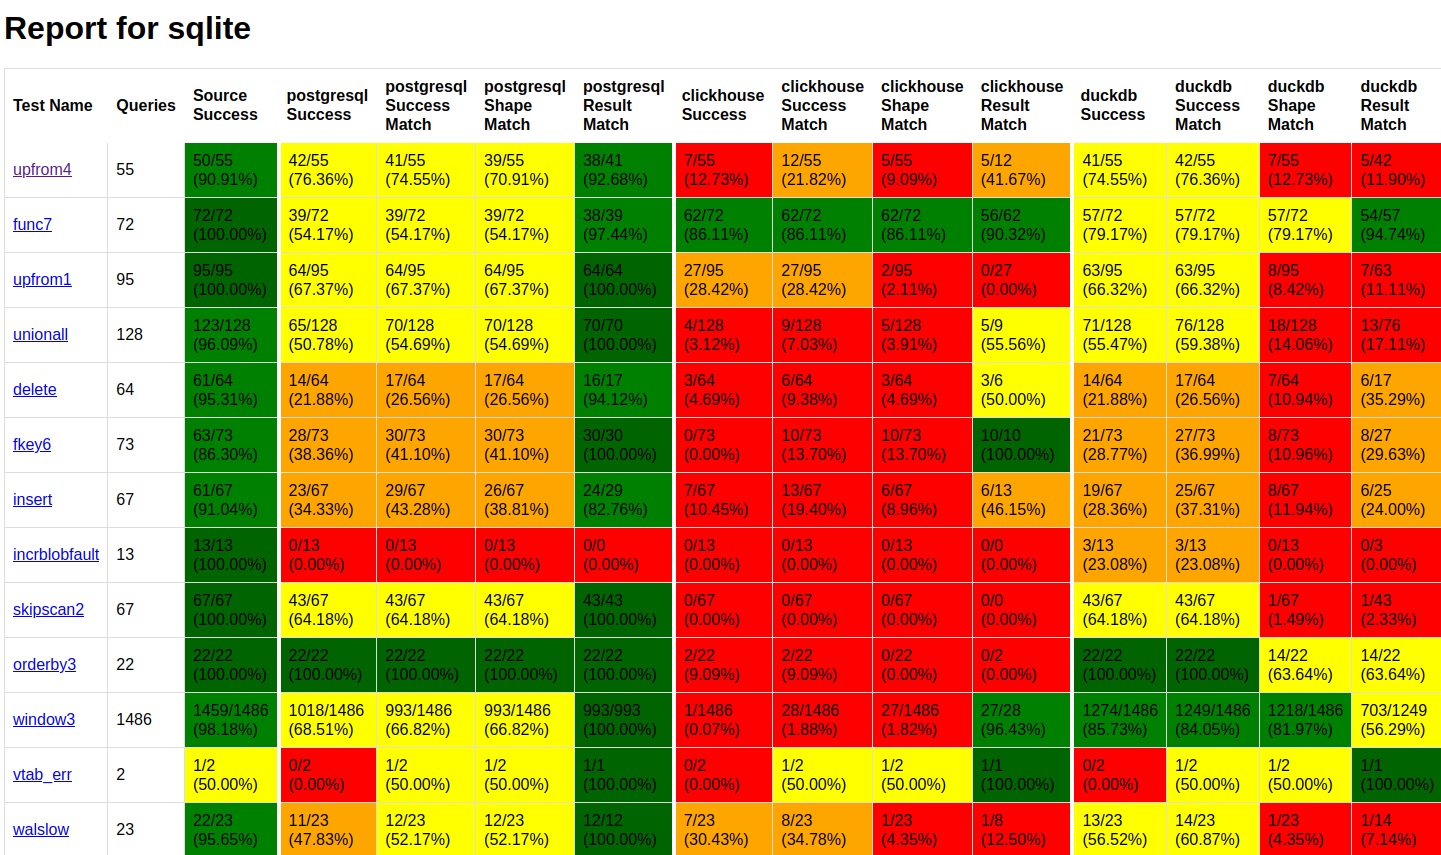
\includegraphics[width=0.7\linewidth]{img/report_01.png}
    \caption{Report snippet 1}
    \label{fig:rep1}
\end{figure}
\begin{figure}[H]
    \centering
    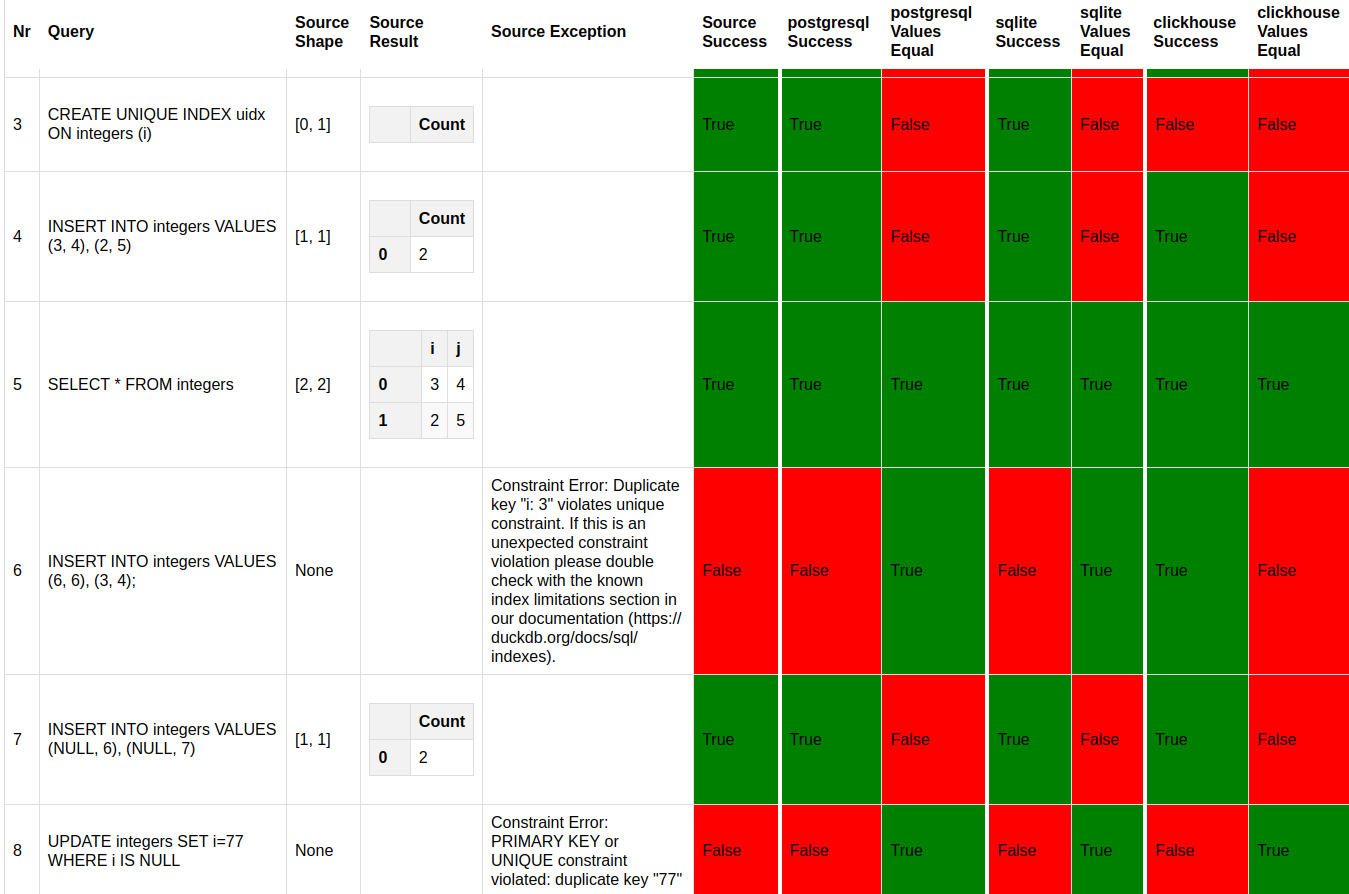
\includegraphics[width=0.7\textwidth]{img/report_02.png}
    \caption{Report snippet 2}
    \label{fig:rep2}
\end{figure}
\begin{figure}[H]
    \centering
    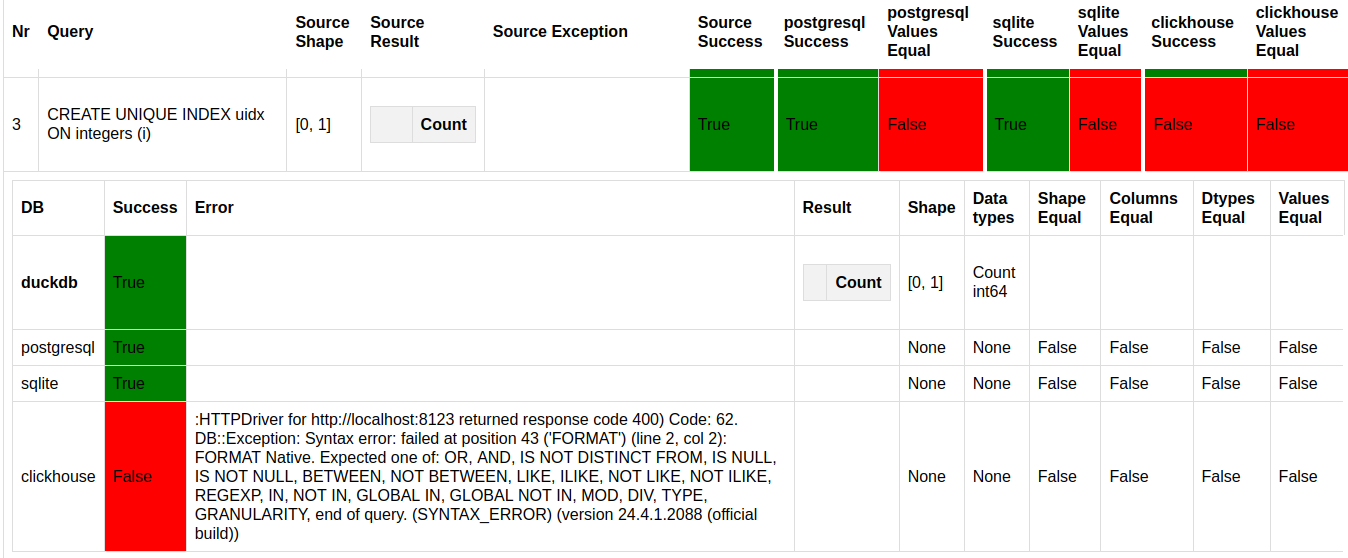
\includegraphics[width=0.7\textwidth]{img/report_03.png}
    \caption{Report snippet 2}
    \label{fig:rep3}
    \vspace{-0.3cm}
\end{figure}

The example view in \autoref{fig:rep1} helps us to quickly identify either such broken tests that we exclude from further evaluation, or to spot errors in our test parser.

In the view in \autoref{fig:rep2} we notice the \texttt{test\_unique\_temp.test} and all the SQL statements contained withing the file and their outcome. Notice for example how for query \#6 and \#8 the expected result does not match and therefore the statement is marked as failed. To view in detail how all DBMS performed on a specific query we can click the query for a detailed view.


By analyzing the passing/failing tests we can draw some conclusions on the functionalities and behaviour of each DBMS.

\subsection{Syntax}
Postgres supports table inheritance through the INHERITS keyword, and from some tests it is obvious that it is the only DBMS to support it, in which all other DBMS return an error upon encountering the INHERITS keyword. Source [\texttt{create\_misc.sql}]

While developing our parser, we encountered an interesting error that was due to us overlooking comments when parsing tests, which led to us discovering that every DBMS, for the exception of SQLite, accepts queries that are empty (or that just contain a comment). 

Furthermore, when running SELECT queries, if we select a column more than once Clickhouse doesn't show the duplicated column while DuckDB opts to add a suffix I eg. \texttt{\_01}, \texttt{\_02} etc to make each column identifier unique.Another  very interesting fact that arises from our analysis is that when using the \texttt{ORDER BY} keyword, PostgreSQL doesn't exhibit case sensitivity when sorting, while all other DBMS clearly sort not based on the alphabetical order but rather on the character value, resulting therefore in capital letters getting sorted in front of small letters. Finally using \texttt{GROUP BY} and \texttt{SORT BY} together with a expression to be evaluated yields very inconsistent results. Source [\texttt{select\_implicit.sql} - \autoref{fig:selectimplicit} ], On the other hand, UNIONS worked very consistently across DBMSs. 

A DuckDB feature that stands out is the ability to perform array indexing inside of queries. This curious feature is unsupported by all other DBMS. [\texttt{test\_list\_index.sql}].


Queries which alter the DB/table schema usually return consistent results, although there are some specific which don't work which often arise when modifying some restricted schema which is usually DBMS specific. (e.g. \texttt{pg\_user}, \texttt{pg\_database}). Source [\texttt{alter.sql}]


\subsection{Data Definition Language (DDL)}
From the tests we noticed that the DBMSs don't all return the same data when executing a successful DDL query (e.g \texttt{CREATE} query), while some return results that are in a different shape.

Generally, Postgres and SQLite tend to return the exact same results. Obviously, the \texttt{SERIAL} data type is a Postgres-specific test, leading Duckdb and Clickhouse to return a syntax error on tests containing that keyword [\texttt{plpython\_schema.test}]. On the same note of Postgres-specific features, the other DBMS clearly do not support table partitioning and adding comments on columns like PostgreSQL does, therefore we are unable to utilize the \texttt{PARTITION} and \texttt{COMMENT} keywords [\texttt{partition\_aggregate.sql}]. On the matter of data types, we noticed that the \texttt{BLOB} data type is only supported by SQLite and DuckDB.


\subsection{Built-in functions}
Clickhouse doesn't handle UTF-8 characters at all, and it is very apparent from some tests which show that Clickhouse does not handle well the variable nature of the UTF-8 encoding. Clickhouse unlike every other DBMSs also has issues in returning the correct length of complex unicode strings that contain special characters and/or emojis.

When running some native Clickhouse tests, we noticed that Clickhouse features a plethora of timestamp-related functions, which are not offered in every other DBMS. We therefore have a wide array of datetime tests failing because such functions are defined only in Clickhouse [\texttt{parse\_datetime\_besteffort\_or\_null\_emptystring.sql}].


\subsection{Boolean handling}

Postgres and Clickhouse are the only ones that have passing queries that use the \texttt{bit} built-in function. In particular, Sqlite and Clickhouse want a different format for specifying binary strings. [\texttt{bit.sql}]. Regarding SQLite, we noticed that the \texttt{BOOL} data type doesn't exist, and therefore it uses integers for representing binary values. Our testing infrastructure performs implicit casting when comparing values, therefore the test still passes [\texttt{bool.sql}]. Additionally all DBMS support the \texttt{ILIKE} comparison operator while SQLite doesn't.


\subsection{Error handling}
A very curious test instance regarding error handling surfaced when running a test which performs division by 0. We can see from the tests that division by 0 is not allowed by Postgres, while it is allowed by other DBMSs. When casting the result to an Integer in a second moment, most DBMS emit then an error.


\subsection{Test suite limitation}

We build the application to be as expandable as possible. Adding new DBMS into the existing infrastructure would require minimal cost. The main time cost would come from the writing of the new parser for the new DBMS. Extending the runner to then evaluate the tests would be minimal.

\section{Future work}
As mentioned before, the tests are not always perfect and may have dependencies that need to be resolved to successfully execute subsequent queries. Detecting and fixing issues after a failed test would be beneficial for thoroughly testing all DBMSs with all test suites. However, this would require an in-depth understanding of each query's purpose and potentially rewriting them. Another task would be to ensure that all tests pass on their own source DBMS, as some queries failed due to missing plugins or data imports that were executed by DBMS-specific test runners.

It would also be interesting to expand our test runner to include more test suites and additional DBMSs. This would allow for a broader comparison of SQL dialects and their differences.

\section{Artifacts}
The public repository of the project is hosted on GitHub \href{https://github.com/BattleRush/AST-SQLDialects-Checker}{https://github.com/BattleRush/AST-SQLDialects-Checker} together with the latest report HTML file and the files to reproduce the results.
% ### Syntax
% - **Postgres**
%   - It shows clearly that INHERITS is a Postgres specific keyword
%     - `create_misc.sql`
%   - By our mistake we found out that inly sqlite accepts queries that are empty (or only contain comments)
%   - When running SELECT queries with duplicated column, Clickhouse doesnt show duplicated column, while DuckDB changes the name of the returned columns such that they have a a different name (i.e postfix *1,* 2 etc)
%   - Implicit nondeterministic ordering. PostgreSQL when sorting is case insensitive, while the other are case sensitive.
%   - When doing a GROUP BY with a SORT BY where the arguments are some form of expression yield different results.
%     - `select_implicit.sql`
% - **Sqlite**
%   - Queries which alter schema of DB generally work, although there are some specifics which dont work whicoh often arise when modifying the svhema which is usually DBMS specific. For example: VIEWS work
%     - `alter.sql`

% ### Data Definition Language (DDL)
% - **Postgres**
%   - Postgres and Sqlite have the exact same results. Test creates tables and indexes. Duckdb and Clickhouse fail because SERIAL is not a valid data type.
%     - `plpython_schema.test`
%   - Other DBMS clearly dont support the PARTITION and COMMENT feature
%     - `partition_aggregate.sql` and `create_table_like.sql`
%   - Some DBMS return no feedback of the successful execution of a CREATE query, while some return results that are in a different shape.
% - **Sqlite**
%   - Sqlite has blob type and DuckDB, while Clickhouse and Postgres fail
%     - `ncrblobfault.sql`

% ### Built-in Functions
% - **Postgres**
%   - Built in functions, SELECT, EXPLAIN
%     - `bloom.sql`
%   - Postgres and Clickhouse are the only ones that have passing queries that use the "bit" built in function.
%     - `bit.sql`
%   - Postgres supports BIT, Duckdb doesn’t. While Sqlite and Clickhouse want a different format for specifying binary strings.
%     - `bit.sql`
%   - Clickhouse by default doesn’t handle UTF-8 characters
%     - `utf8.sql`
% - **Sqlite**
%   - BOOL doesn’t exist and it uses integers, but in our testing we perform implicit casting for comparison
%     - `bool.sql`
% - **Clickhouse**
%   - Built-in timestamp/date completely fail on others cause they are specific only to clickhouse.
%     - `parse_datetime_besteffor_or_null_emptystring.sql`
%   - UNIONS work across all DBMSs
%     - `h_union_al.test`
% - **Duckdb**
%   - Duckdb supports array indexing, while other don't.
%     - `test_list_index.test`
%   - All DBMS support ILIKE comparison while sqlite doesn’t.
%     - `like_unicode_test.sql`

% ### Boolean Handling
% - **Postgres**
%   - Boolean works the same way, although other DBMSs sometimes perform implicit casting when answering with the result set
%     - `bool.sql`
% - **Sqlite**
%   - BOOL doesn’t exist and it uses integers, but in our testing we perform implicit casting for comparison
%     - `bool.sql`

% ### Error Handling
% - **Postgres**
%   - This test checks for correct throwing of errors. We can see that for example, division by 0 is not allowed by postgres, while it is allowed on all other DBMSs, with clickhouse returning inf, duckdb NaN and sqlite None. Instead, when division by 0 is casted to integer, most DBMSs give out an error.
%     - `errors.sql`

% ### Data Types
% - **Postgres**
%   - Postgres and Sqlite have the exact same results. Test creates tables and indexes. Duckdb and Clickhouse fail because SERIAL is not a valid data type.
%     - `plpython_schema.test`
% - **Sqlite**
%   - Sqlite has blob type and DuckDB, while Clickhouse and Postgres fail
%     - `ncrblobfault.sql`

% ### UTF-8 and Unicode Handling
% - **Postgres**
%   - Clickhouse by default doesn’t handle UTF-8 characters
%   - When creating a table Sqlite and Duckdb assume NON NULLness in which we cannot insert fewer values than columns, unlike Postgres which allows to do so.
%     - `utf8.sql`
% - **Duckdb**
%   - Clickhouse unlike every other DBMS has issues in returning the correct length of complex unicode strings that contain special characters and/or emojis.
%     - `test_complex_unicode.sql`
%   - In general UTF 8 and clickhouse don’t go along

% ### Math Functions
% - **Sqlite**
%   - Most math-based functions behave the same way, including rounding, pi, etc. Our tester is more lenient with these tests as we preset a certain precision when checking for equality.
%     - `func7.test`

% ### Data Manipulation Language (DML)
% - **Sqlite**
%   - DELETE statements tend to behave the same way. PRAGMA is quite unstable as its results are not consistent across DBMSs
%     - `delete.sql`

% ### Order By
% - **Sqlite**
%   - Order by statement is generally consistent.
%     - `orderby3.sql`

% ### Views and Materialized Views
% - **Postgres**
%   - Materialized views, again fails
%     - `tid.sql`
% - **Sqlite**
%   - Queries which alter schema of DB generally work, although there are some specifics which don't work which often arise when modifying the schema which is usually DBMS specific. For example: VIEWS work
%     - `alter.sql`

% ### WITH RECURSIVE
% - **Sqlite**
%   - While Clickhouse fails to interpret WITH RECURSIVE statements, all the others do.
%     - `walslow.test`





% 3. Final Report (due 26.05):
% - incorporate feedback and polish the previous sections.
% - complete the project report with the experimental results.
% - submit the project report and the artifact.
% - the artifact should include your implementation and the experimental results with a README.
% - the README should specify how the artifact supports the claims in the project report.
% - we will check the artifact according to the README.

% 3. Final Report (30 points):
% - writing quality (10 points): Is the project clearly presented?
% - results (10 points): How good are the results?
% - completeness (10 points): Have students finished the approach/experiments of the proposal?


\end{document}
